\section{Methods}
Despite progress in counterfactual explanations for \gls{tsc} or \gls{tsf} \cite{theissler_explainable_2022, rojat_explainable_2021}, Table~\ref{table:xai-survey} indicates a notable gap in addressing \gls{tser} tasks. In fact, to the best of our knowledge, there currently does not exist any method for (deep learning) based explainable extrinsic regression. This work introduces novel methods for explainable \gls{tser}. 
We begin by precisely defining \gls{tser} ~(cf. Section~\ref{sec:methods:tser}). 
Afterward, we showcase our reasoning behind the choice of counterfactuals to explain \gls{tser}.
Furthermore, we outline a framework for the transformation of explainable counterfactual-based methods from classification to extrinsic regression~(cf. Section~\ref{sec:methods:tser_threshold}) and introduce definitions for desired properties for counterfactuals in \gls{tser}~(cf. Section~\ref{sec:methods:tser}) adopted from prior work~\cite{delaney_instance-based_2021}. We apply this framework to adopt four \gls{tsc} methods for \gls{tser}~(Section~\ref{sec:methods:tser_adoption}), namely 
\begin{enumerate}
    \item \gls{wachter} ~(Section~\ref{sec:methods:wachter})
    \item \gls{nunr}~(Section~\ref{sec:methods:nun})
    \item  \gls{dbar}~(Section~\ref{sec:methods:dbar})
    \item \gls{tsevor}~(~Section~\ref{sec:methods:tsevo})
\end{enumerate}
Lastly, we evaluate the four methods on the task of biological age estimation to derive recommendations for individuals to improve their health~(cf. Section~\ref{sec:methods:experiments}).


\label{sec:methods}
\subsection{\gls{tser} and User Explainability}
\label{sec:methods:tser}

\gls{tser} is a regression task that learns the mapping from time series data to a scalar value \cite{tan_time_2021}. We formally define \gls{tser} by Definition~\ref{def:tser}.
\begin{definition}
\label{def:tser}
Let $x=\left[x_{1}, \ldots, x_{T}\right] \in \mathbb{R}^{N \times T}$ be a uni- or multivariate time series, where $T$ is the number of time steps, and $N$ is the number of features. Let $x_{i,t}$ represent input feature $i$ at time $t$, and $y$ denote the output. Then, the regression model $f : x \rightarrow y$ returns an extrinsic continuous variable, with $f$ considered a "black box" — i.e., no access to the inner workings of the model is available, and only the result $y$ is observable.
\end{definition}

In Section~\ref{sec:related-work}, we discovered numerous techniques for explaining time series data. Perturbation-based, backpropagation-based, and attention-based methods have one thing in common: They show which part of the time series influences the model's output. While this is useful for the developer or a field expert, a user may not know how to interpret this explanation. When aiming for continuous health assessment, the explainability method should focus on \textit{actionability}, i.e., it should be able to show the user how to change his behavior to improve the model's output, meaning that the technique should have a local scope and target the user. Another criterion to consider is the model-specificity or model-agnosticism of an explainable technique. Indeed, as most model-specific methods focus on models used for classification, and as we explore different black-box model architectures to perform biological age estimation, we considered only post-hoc, model-agnostic methods. Model-agnostic methods allow us to explain existing models without modifying them for transparency. However, this approach does not come without drawbacks: Post-hoc methods can result in explanations based on misconceptions learned by the model rather than actual knowledge from the data \cite{laugel_dangers_2019}. From the different already implemented techniques available for \gls{tsc} (see Table \ref{table:xai-survey}), the explanation method that would provide local, user-targetted explanations while being model agnostic is called \textit{\gls{cf}}. The following subsections define how to adapt existing counterfactual methods for \gls{tsc} to \gls{tser}.
 
\subsection{Counterfactual in \gls{tser} via thresholding and its Desired Properties} 
\label{sec:methods:tser_threshold}
The common goal of counterfactual approaches is to provide an explanation via counter-examples given a time series $x$, called a query, and a model $f$. In classification scenarios, counter-examples allow users to understand why a classifier-model $f$ predicts a label $y$ for data point $x$ instead of a counterfactual class $y^{c f}$ \cite{wachter_counterfactual_2018}. However, in the case of extrinsic regression, we do not have classes as we are predicting a continuous value and not a categorical value. Using only an inequation such as $y \neq y^{c f}$  would not work since the difference between the query and the counterfactual labels could be infinitely small, providing insufficient information. Yet, we can enforce a minimal change required for a data point to be counterfactual, and this is done via thresholding: we assume that for each $x$, a counterfactual sample $x^{c f}$ can be computed that is close to $x$, but with a minimum prediction difference larger than a certain threshold $|y - y^{c f}| > \varepsilon$\footnote{\textbf{Important note:} In the specific case of biological age estimation, as we want to find a healthier patient, we are looking to decrease the \gls{ba} of the patient. Therefore, we are only interested in counterfactuals whose predicted values are lower than the patients' \gls{ba} by a certain margin (e.g., at least three years younger).}. A counterfactual should meet a few desired properties to be considered a relevant explanation for a user.
When dealing with time-series data, we typically consider the following four properties \cite{delaney_instance-based_2021}:
\begin{enumerate}
    \item Validity~(Def.~\ref{def:validity})
    \item Proximity~(Def.~\ref{def:proximity})
    \item Sparsity~(Def.~\ref{def:sparsity})
    \item Plausibility~(Def.~\ref{def:plausibility})
\end{enumerate}

Let $x=\left[x_{1}, \ldots, x_{T}\right] \in \mathbb{R}^{N \times T}$ be a uni- or multivariate time series or so-called query, where $T$ is the number of time steps, $N$ is the number of features, $x^{cf}$ a counterfactual, and $\mathcal{X}$ the input space.
Then, for a fixed $\varepsilon$, the set of valid counterfactuals denoted as $\mathcal{S}$ is defined by Definition~\ref{def:validity}.

\begin{definition}[Validity of the counterfactual]
\label{def:validity}
We define the validity property for TSER as:
$$\mathcal{S} \doteq \{x \in \mathcal{X}:\valid{x}{x^{c f}}\}$$
\end{definition}
This equation defines a set of accepted counterfactual labels for each query. It requires that the distance between the query label and the counterfactual label is larger than the threshold $\varepsilon$ but does not exceed twice the $\varepsilon$ value. The upper limit is because on the label axis, the threshold defines an area around the query where samples are not considered counterfactuals as they are too close to the query. It mimics the behavior of a class; if we move on the label axis from the query label by a distance $\varepsilon$, we are in the counterfactual area, i.e., in another class. If we move again by the same $\varepsilon$ distance, we are no longer in this counterfactual area. We are too far from the query. The latter limit is set to ensure that the  \gls{cfe} does not differ too much from the original query \cite{spooner_counterfactual_2021}.
For example, applied to biological age estimation, if we let the patient query be 56 years old and $\varepsilon = 3$, then a valid counterfactual has a label between 50 and 53 years old. A 55-year-old counterfactual is considered too close to the query to be relevant, and the lower limit ensures that a 20-year-old counterfactual is not suggested, as he would be too distant from the query.   

\begin{definition}[Proximity of the counterfactual]
We characterize the proximity property for TSER as follows:
\begin{equation}
\begin{aligned}
\min_{x^{cf}} \quad & d(x, x^{c f})\\
\mathrm{s.t.} \quad & \valid{x}{x^{c f}}\\
\end{aligned}
\end{equation}
\label{def:proximity}
\end{definition}
This property ensures that the resulting $x^{c f}$ is a proximate instance to the query \cite{mothilal_explaining_2020}. Proximity refers to the distance between the query instance $x$ and the counterfactual instance $x^{c f}$, calculated as a distance measure $d$ between $x$ and $x^{c f}$. A commonly used metric for the distance between two time series is the \gls{dtw} distance \cite{muller_dynamic_2007}.
% In the case of biological age estimation, it ensures that the query and the counterfactual have related \gls{pa} in terms of intensity.

\begin{definition}[Sparsity of the counterfactual]
We define the sparsity property for TSER as follows:
\begin{equation}
\begin{aligned}
\min_{x^{cf}} \quad & \sum_{i=1}^{N} \sum_{t=1}^{T} \mathbbm{1}_{|x_{i, t}-x_{i, t}^{c f}| \neq 0}\\
\mathrm{s.t.} \quad & \valid{x}{x^{c f}}\\
\end{aligned}
\end{equation}
\label{def:sparsity}
\end{definition}
Sparsity refers to the number of changes in data points between $x$ and $x^{c f}$ \cite{mothilal_explaining_2020}. This key property forces a \gls{cfe} method to make human-interpretable changes.
When enforcing the sparsity property, \gls{cfe} methods strive to alter the fewest variables necessary to achieve user-interpretable solutions.
Another constraint specific to time series data is that not only the fewest number of variables should change, but the changed variables should be in continuous subsequences of the original time series. Each counterfactual method implements a different technique to overcome this constraint.

\begin{definition}[Plausibility of the counterfactual]
We define the plausibility property of counterfactuals in the context of TSER as follows:
\begin{equation}
\begin{aligned}
 \quad & x^{c f} \sim D\\
\mathrm{s.t.} \quad & \valid{x}{x^{c f}}\\
\end{aligned}
\end{equation}
\label{def:plausibility}
\end{definition}
A counterfactual $x^{c f}$ is plausible if it could have been drawn from the data $D$ \cite{laugel_dangers_2019}. The plausibility property ensures that the post-hoc explanation method produces justified explanations. This property is verified by looking at the neighbors' explanation labels and analyzing whether they are close to the explanation's label. A counterfactual with a label far away from his neighbor's label is considered unjustified. In biological age estimation, a justified counterfactual has neighbors in the same age range, i.e., the distance between the counterfactual's label and the neighbor's label is below the threshold $\varepsilon$. 


\subsection{Adoption of methods for time-series extrinsic regression}
\label{sec:methods:tser_adoption}
Given our prior definitions of desired properties for counterfactuals in \gls{tser}, we describe our adoption of four methods of \acrshort{tsc} to \acrshort{tser}. Based on its results, we chose \gls{tsevo} first, as it seemed to be the more promising approach. Then we adapted Wachter, \gls{nun} and \gls{dba} to compare and put in perspective \gls{tsevo}'s results. In the following sections, we present their adoption chronologically.   

\subsubsection{\gls{wachter}-\gls{cf}}
\label{sec:methods:wachter}
The first candidate for the adoption of \gls{cfe} for \gls{tser}  is Wachter et al. \cite{wachter_counterfactual_2018} (2018). Wachter's approach involves minimizing an equation through gradient descent that combines validity~(cf.~Definition~\ref{def:validity}) and proximity~(cf.~Definition~\ref{def:proximity}) properties. To adapt Wachter's method for \gls{tser}, we replace the classifier model and introduce the threshold criterion~(cf. Section~\ref{sec:methods:tser_threshold}) while the distance function remains unchanged.
Adapting Eq. \ref{eq:wachter}~(cf. Section~\ref{sec:related-work:counterfactual_explanations}) leads to the following : 
\begin{equation} \label{eq:wachteR-cf}
\arg \min _{x^{\prime}} \max _{\lambda} \lambda\left(f_{w}\left(x_{i}\right)-\varepsilon -f_{w}\left(x^{\prime}\right)\right)^{2}+d\left(x_{i}, x^{\prime}\right)
\end{equation}
The main adaptations reside in that $f_{w}$ now denotes a black-box extrinsic regression model, and a threshold $\varepsilon$ is introduced. 

\subsubsection{\gls{nunr}-\gls{cf}}
\label{sec:methods:nun}
The second candidate for \gls{cfe} for \gls{tser} is the \gls{nun} as counterfactuals \cite{nugent_gaining_2009} (2009), and later adapted to time series data by Delaney et al.~\cite{delaney_instance-based_2021} (2021). In a classification setup, the \gls{nun} method aims to find the closest instance in the dataset that is classified differently than the query. It works by creating a reference set containing all instances in the dataset with the target classification or a different classification than the query. Then, the \gls{nun}-\gls{cf} algorithm computes the \gls{nns} of the query that are in the reference set, obtaining the \gls{nuns}. The \gls{nns} are computed using $KNeighborsTimeSeries$ \cite{tavenard_tslearn_2020}.
We must only modify how the reference set is defined to adapt the \gls{nun}-\gls{cf} algorithm to the regression setup.
\begin{definition}[Reference set]
    \label{def:ref-set}
    % \textbf{Reference set} \\
    The reference set is a subset of all known data $D$ with a valid prediction under def. \ref{def:validity}.
    \[
        R = \{z \in D : \valid{x}{z}\}
    \]
\end{definition}
With \gls{nunr}-\gls{cf}, if a \gls{nun} exists, it is guaranteed that the found counterfactual is in the data distribution, as it is an existing sample~(cf.~Def.~\ref{def:plausibility}) and valid~(cf.~Def.~\ref{def:validity}). The proximity~(cf.~Def.~\ref{def:proximity}) of the counterfactuals will be minimized among the existing valid samples, but as shown in previous work \cite{delaney_instance-based_2021, hagen_dice_2020}, the \gls{nun} is not necessarily close to the model decision boundary, and it is possible to find more proximate counterfactuals by mutating the \gls{nun} towards the decision boundary. These mutations are typically done by perturbing the query time series on areas where the query and the \gls{nun} disagree. Another issue is that \gls{nuns} are not sparse; in the context of biological age estimation, the \gls{nunr}-\gls{cf} algorithm locates a physical activity that closely resembles the query's physical activity but is performed by a different individual and slightly varies at each timestamp.

\subsubsection{\gls{dbar}-\gls{cf}}
\label{sec:methods:dbar}
The third method we consider is called \gls{dba}-\gls{cf} and was proposed by Delaney et al. \cite{delaney_instance-based_2021} in 2021. The main idea is to bring the found \gls{nun} closer to the decision boundary by averaging between the query and the \gls{nun}. Originally, Forestier et al. \cite{forestier_generating_2017} (2017) proposed \gls{dba} to augment time-series datasets. \gls{dba} is used to compute the average between time series. The concept behind \gls{dba}-\gls{cf} is to achieve a weighted average between the query and the \gls{nun}, starting with all the weight on the query and then iteratively moving the weight towards the \gls{nun} until the decision boundary is reached.
\subsubsection{\gls{tsevor}-\gls{cf}}
\label{sec:methods:tsevo}
\gls{tsevo} is a technique that combines time series perturbation approaches from the recent work\cite{guilleme_agnostic_2019} and \cite{mujkanovic_timexplain_2023} with a genetic algorithm for multi-objective optimization \cite{dandl_multi-objective_2020}. This technique allows the creation of model-agnostic counterfactual explanations for uni- and multivariate classification problems.
% Unlike previous techniques described in \cite{delaney_instance-based_2021}, \cite{guilleme_agnostic_2019}, and \cite{mujkanovic_timexplain_2023}, \gls{tsevo} does not require an advanced decision regarding the transformer to be made.

\gls{tsevo} tackles the challenge of finding a counterfactual that meets the four key properties validity \ref{def:validity}, proximity \ref{def:proximity}, sparsity \ref{def:sparsity} and plausibility \ref{def:plausibility}. To achieve this, \gls{tsevo} treats each property as an objective to optimize, forming a multi-objective optimization problem. We define below how the properties are transformed into objectives in the setting of \gls{tser}. 

\begin{definition}[Multi-Objective Problem]
$O_{1}$ is derived from def. \ref{def:proximity} by applying \gls{mae} as distance function $d$ \cite{mothilal_explaining_2020}, \cite{wachter_counterfactual_2018}.
$$O_{1}(x, x^{c f})=\frac{1}{NT} \sum_{i=1}^{N} \sum_{t=1}^{T}|x_{i, t}-x_{i, t}^{c f}|$$ $O_{2}$ is consistent with def. \ref{def:sparsity}.
$$O_{2}(x, x^{c f})=\frac{1}{NT} \sum_{i=1}^{N} \sum_{t=1}^{T} \mathbbm{1}_{|x_{i, t}-x_{i, t}^{c f}| \neq 0}$$ $O_{3}$ denotes the normalized output distance.
$$O_{3}(x, x^{c f})=(f(x) - f(x^{c f})-\varepsilon) / \varepsilon$$ Combining the desired properties leads to the following multi-objective problem $O$:
\begin{equation}
\begin{aligned}
\min_{x^{cf}} \quad & O(x, x^{cf}):=(O_{1}(x, x^{c f}), O_{2}(x, x^{c f}), O_{3}(x^{c f}))^T\\
\mathrm{s.t.} \quad & \valid{x}{x^{c f}}\\
\end{aligned}
\end{equation}
\end{definition}
The multi-objective optimization follows the steps described in the original \gls{tsevo} publication \cite{hollig_tsevo_2022}.
In summary, a population of $n$ individuals is initialized, where each individual represents a potential counterfactual.
The individuals are evaluated with respect to their objectives score.
For $g$ generations, the evolution algorithm selects the best individuals in the population according to how they fulfill the different objectives. Depending on a certain probability, it performs crossover and/or mutates them. For the mutations, we used the authentic opposing information mutation, first introduced by Guilleme et al. \cite{guilleme_agnostic_2019}, which is based on the assumption that interpretable values of time series can exhibit shapes (e.g., peaks) that are easily understandable to humans.
To use those shapes included in a reference set $R$~(cf.~Def.~\ref{def:ref-set}), we draw a random sample $r \in R$. 
Both $r$ and the selected individual $\lambda_i$ are segmented with window size $w_i$, resulting in $S(r)$ and $S(\lambda_i)$. The mutation then draws a random segment index $s \in [ 0,|S(r)|-1]$ and replaces the drawn slice $S(\lambda_i)[s]$ with the slice $S(r)[s]$ from the replacement time series. The concept of crossover in genetic algorithms is utilizing the search space by merging the genetic material of high-performing individuals \cite{mitchell_introduction_1998}.
The reference set is used in the evolution algorithm to mutate the individuals. It ensures that the mutated individuals stay in the data manifold. Note that this is meant to achieve the plausibility property~(cf.~Def.~\ref{def:plausibility}) by design, as this property was not expressed as an objective.

\subsection{Experimental Evaluation}
\label{sec:methods:experiments}
Our work was motivated by the findings of Pyrkov et al. \cite{pyrkov_extracting_2018} and Rahman et al. \cite{rahman_deep_2019}, who showed that deep learning models could estimate the biological age of a patient from his physical activity. Once we predict the biological age, we can use counterfactual explanations to give feedback to the patient.

The following Sections describe our efforts to reproduce prior work to train models for biological age estimation, enabling us to test our \acrshort{cfe} methods. For the training and data generation, we followed the same steps as described in prior work in Pyrkov et al. \cite{pyrkov_extracting_2018}, Rahman et al. \cite{rahman_deep_2019}, and Shim et al. \cite{shim_wearable-based_2023}. Figure \ref{fig:pipeline} shows an overview of the whole pipeline, from data generation to providing recommendations.

\begin{figure}
    \centering
    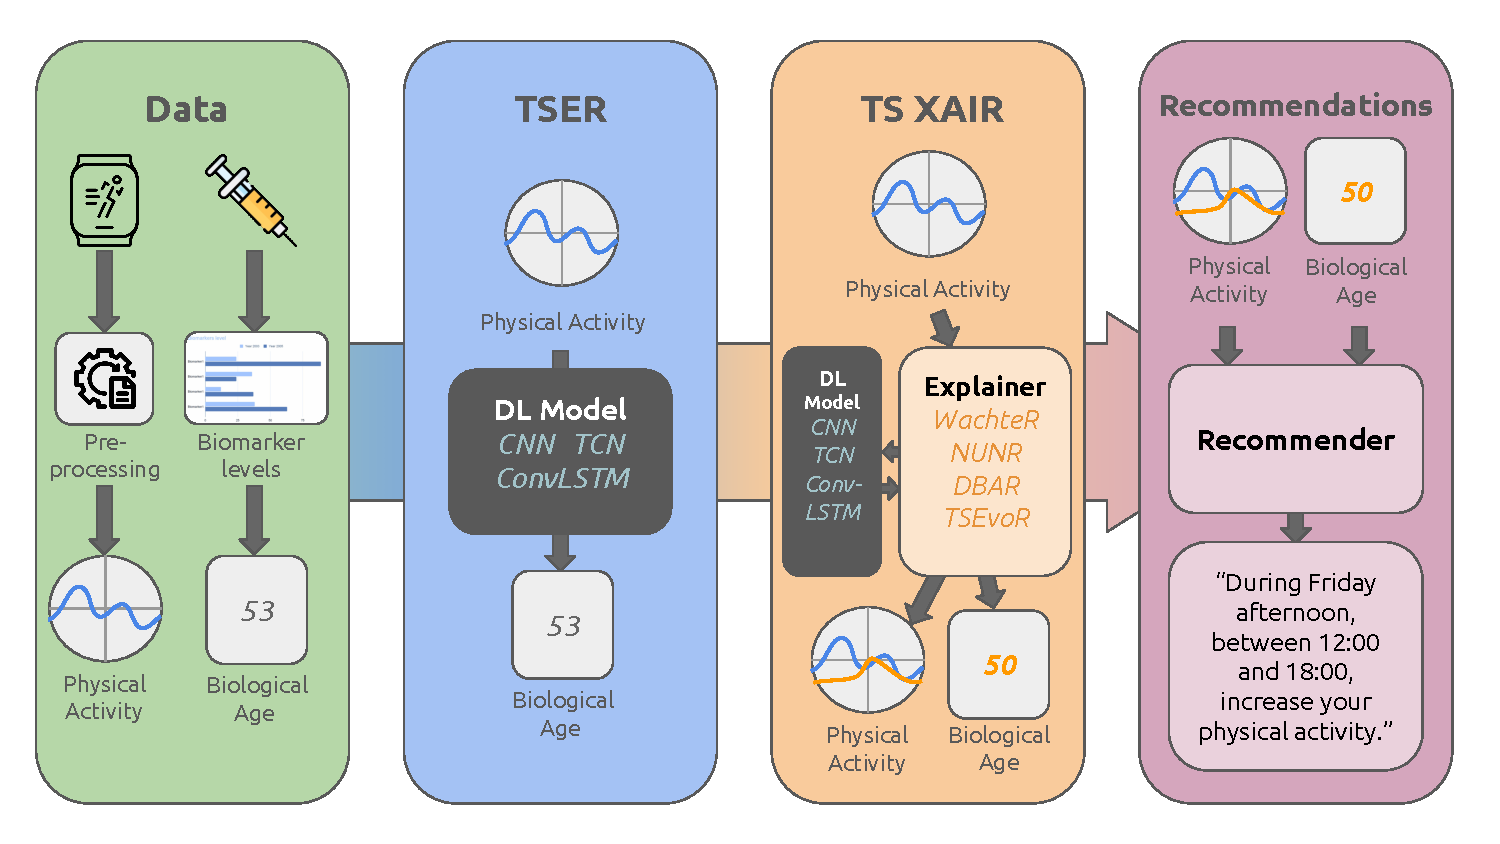
\includegraphics[width=1\linewidth]{images/pipeline.pdf}
    \caption{Pipeline: From data preprocessing to physical activity recommendations.}
    \label{fig:pipeline}
\end{figure}

\subsubsection{Physical Activity}
\textbf{Description} We used physical activity data recorded during the \gls{nhanes} from 2003 to 2004 \cite{cdc_nhanes_2003} and from 2005 to 2006 \cite{cdc_nhanes_2005}. 
\gls{nhanes} uses a complex sampling design to survey non-institutionalized members of the US population.
A subset of \gls{nhanes} participants recorded their activity data. During the survey, participants' physical activity is tracked for seven continuous days using a physical activity monitor\footnote{The monitor used was the ActiGraph AM-7164; ActiGraph, Pensacola, FL, USA} to record \textit{activity counts} sampled every minute. 
The participants wear the monitors on the right hip using an elastic belt.
The datasets included 14'631 participants, with 7'176 in 2003-2004 and 7'455 in 2005-2006.
\textbf{Filtering} The filtering steps are based on prior work done on biological age estimation~\cite{pyrkov_extracting_2018, rahman_deep_2019, shim_wearable-based_2023}. First, we removed outliers with abnormally low ($< 50$) or high ($>5000$) mean activity count. Then, we removed patients with less than 10'080 ($= 7 \times 24 \times 60$) activity counts, corresponding to one measurement every minute for seven days. Also, we only considered days where the participant was active for more than 200 minutes. Therefore, we filtered out participants who had less than four days of meeting this criteria. This filter resulted in a total of 9,591 individuals.
\textbf{Transformation} To handle the noisy and outlier-filled nature of the time-series human locomotor data, we first needed to apply some basic data transformation operations, such as smoothing.
The physical activity intensity $(pa_{intensity})$ values range over a large magnitude and are always positive, so we applied log transformations to the data, as suggested by Rahman et al. \cite{rahman_deep_2019}.
However, since the original data contains some $0$ values, we added a negligible value ($1$) before applying log transformations.
The first transformation is a Box-Cox \cite{box_analysis_1964} transformation with $\lambda = 1$, which is equivalent to a simple log transformation (other values of $\lambda$ were investigated by Rahman et al. \cite{rahman_deep_2019}).
Then, a second log transformation is computed. Since the data is a sequential time series of seven days, we applied moving averages on the data with different window sizes and an \gls{ema}. 
\begin{equation}
    pa_{log} = \log(BoxCox(pa_{intensity} + 1) + 1)
\end{equation}
\begin{equation}
    pa_{ema}^i = 
    \begin{cases}
      pa_{log_i}, & \mathrm{if}\ i=1 \\
      \alpha pa_{log_i} + (1 - \alpha) pa_{log_{i-1}}, & \mathrm{otherwise}
    \end{cases}
\end{equation}

We used $\alpha = \frac{1}{N+1}$ and $N=35$, as it was reported to be the best window size by Rahman et al. \cite{rahman_deep_2019}.

\subsubsection{Biological Age}
We used the \gls{nhanes} 2003-2006 anthropometric and bio-marker datasets to compute each patient's biological age \cite{kwon_toolkit_2021}.
The biomarker dataset contained information on albumin, alkaline phosphatase, blood urea nitrogen, uric acid, cholesterol, creatinine~\cite{cdc_biopro_d_2005}, C-reactive protein~\cite{cdc_crp_d_2005}, body mass index~\cite{cdc_bmx_c_2003}, glycohemoglobin~\cite{cdc_l10_c_2003}, systolic and diastolic blood pressure~\cite{cdc_bpq_c_2003}, lymphocyte percentage, mean cell volume and white blood cell count~\cite{cdc_l25_c_2003}.
% BIOPRO_D
% albumin
% alp =  Alkaline Phosphatase
% bun =  blood urea nitrogen
% uap =  uric acid
% totchol = Cholesterol
% lncreat = Creatinine (mg/dL) 
% 
% CRP_D
% crp = C-reactive protein
% 
% BMX_C
% bmi = Body Mass Index
% 
% L10_C
% hba1c = Glycohemoglobin 
% 
% BPQ_C
% sbp = Systolic and diastolic blood pressure
% 
% L25_C
% lymph = Lymphocyte percent
% mcv = Mean cell volume
% WBC = White blood cell count
Then, we used the Klemera-Doubal method \cite{klemera_new_2006} to compute a mapping between the biomarkers information and the biological age. We retained only patients aged between 18 and 85. As a result, we obtained a dataset of 10,184 patients along with their corresponding biological age.
Lastly, we combined the physical activity dataset with the biological age datasets, resulting in 7'222 matched patients. Not all patients in the physical activity dataset were included in the biomarker dataset, hence the lower total number of patients. We split the combined dataset into training ($65\%$), validation ($25\%$), and testing ($10\%$) sets, yielding 4'694, 1'805 and 723 patients, respectively.
\subsubsection{Deep Learning models for Biological Age Estimation}
Using physical activity data to predict biological age is an example of a \gls{tser} task. In our scenario, we trained and tested three different models to predict biological age from physical activity data: 

\begin{enumerate}
    \item A \textit{\gls{cnn}} suggested by Pyrkov et al. for biological age estimation \cite{pyrkov_extracting_2018}
    \item A \textit{\gls{convlstm}} proposed by Rahman et al. for biological age estimation \cite{rahman_deep_2019}.
    \item A \textit{\gls{tcn}} \cite{lea_temporal_2016, bai_empirical_2018} network. 
    \end{enumerate}
To the best of our knowledge, the \gls{tcn} model has not yet been tested for biological age estimation in prior work. It was included in the evaluation in this work because recent literature indicates that \gls{tcn} models can achieve state-of-the-art results on time series tasks while often being less complex than \gls{lstm} models~\cite{bai_empirical_2018}.
Each model requires a different data representation: The \gls{cnn} takes as input a flat vector of 10'080 values, \gls{convlstm} uses a complex 3D representation ($60, 24, 7$), and \gls{tcn} falls in between the two, taking vectors of shape $(7, 1440)$, where the days are treated as features. We trained all models on the training data for \gls{convlstm} and \gls{cnn}; we used the steps and hyperparameters described by Rahman et al.~\cite{rahman_deep_2019} and Pyrkov et al.~\cite{pyrkov_extracting_2018} respectively.
                 % num_channels: list[int] = [128]*10,
                 % kernel_size: int = 4,
                 % dropout: float = 0.2,
                 % num_timestamps: int = PhysicalActivity.NumberOfMinutesPerDay,
                 % patience: int = 10,
                 % verbose: bool = False,
                 % delta: int = 0,
                 % % save_model: bool = True):
The \gls{tcn} has ten layers of 128 channels each; we used a kernel size of 4 and a dropout of 0.2. We trained the model for 100 epochs, with a learning rate 0.0001, and we chose the best model according to the \gls{mse} loss. We recorded two other metrics, which are the \gls{mae}, which gives a more intuitive comprehension of the error of the model than the \gls{mse}, and the Pearson correlation, which indicates the strength of the linear association between the physical activity and the biological age. 

\subsubsection{Explainable Biological Age Estimation}
Utilizing our counterfactual adaptations \gls{wachter}, \gls{nunr}, \gls{dbar} and \gls{tsevor}, we generated counterfactuals with threshold $\varepsilon=3$~(cf.~Section~\ref{sec:methods:tser_threshold}) for each sample of the 723 samples in the test set using the three different models.
For \gls{wachter}, we defined a loss function from eq. \ref{eq:wachteR-cf}:
\begin{equation}
    \label{eq:wachter-loss}
    \text{LOSS} = \lambda\left(f_{w}\left(x_{i}\right)-\varepsilon -f_{w}\left(x^{\prime}\right)\right)^{2}+\left(1-\lambda\right)d\left(x_{i}, x^{\prime}\right)
\end{equation}
and $x^{\prime}$ was initialised  to $x_{i}$ (we also attempted random initialization). 
Using the L1-Norm as distance function $d$, we then performed a gradient descent using the ADAM \cite{kingma_adam_2017} optimizer for $n=100$ iterations for each lambda $\lambda$ and increased lambda by $0.05$ if no valid (Def. \ref{def:validity}) counterfactual is found. The valid counterfactual with the smallest loss~(Eq.~\ref{eq:wachter-loss}) is returned. If no valid counterfactual is found after trying out all lambdas, we return the counterfactual with the smallest corresponding loss.
For \gls{nunr}, once the reference set is adapted (see \ref{def:ref-set}), the remainder of the algorithm is the same as in a classification setting.
For \gls{dbar}, we retrieved the \gls{nun} and performed a weighted sum: 
\begin{equation}
    x^{cf} = DBA(\beta x_{query}, (1-\beta)x_{NUN})
\end{equation}
We chose to run $10$ iterations, increasing $\beta$ by $0.01$ at each iteration and returning $x^{cf}$ as soon as it is valid. 
For \gls{tsevor}, we used the genetic algorithm over 50 generations and applied mutation to the individuals using the authentic opposing information transformer, as implemented by Guillemé et al. \cite{guilleme_agnostic_2019}.

\subsubsection{Habits recommendations}
The generated counterfactuals depict time series plots of recommended physical activity data. Presenting this data to potential patients allows them to interpret what actions they should take to improve their biological age. However, different patients might interpret the counterfactuals differently. 
We designed a system that provides the patient with highly interpretable text feedback to give a more concrete, text-based recommendation. This feedback contains a few sentences or \textit{recommendations} on how to adjust the activity based on the generated counterfactuals. Each day is separated into four parts of six hours each to generate a recommendation $R$:
\begin{center}
    \textit{Night, Morning, Afternoon,} and \textit{Evening}.
\end{center}
For each part $p$, we compute the mean value of the query's physical activity $mean_q$ and the mean of the counterfactual's physical activity $mean_{cf}$. We assume that the obtained means represent a percentage activity on a scale from \textit{No Intensity $(0\%)$} to \textit{Very High Intensity $(100\%)$}. This representation allows us to interpret the difference between $mean_q$ and $mean_{cf}$ as a 
 percentage change. Concretely, this percentage change ($Percentage_{change}$) is defined as follows, where MAX ACTIVITY INTENSITY denotes the maximum value of the intensity of the counterfactual and the query.

% One issue to take into account is that if the query mean is close to zero, for example, 0.1, and the counterfactual mean is, for example, 2, then the change percentage is $ \frac{2 - 0.1}{0.1} * 100 \eq 1900\%$ which is not very intuitive
\begin{equation}
    Percentage_{change} = \frac{mean_{cf} - mean_{q}}{\text{MAX ACTIVITY INTENSITY}} \times 100
\end{equation}
Using our approach, we generate several maximum $n$ recommendations to the user and only include recommendations suggesting a minimal percentage change of at least $p$\%, with $n$ and $p$ being configurable parameters.
\newpage

% \subsubsection{Qualitative Evaluation with Social Science}
% Spreitzer et Al. \cite{spreitzer_evaluating_2022} (2022) examined the practicality of counterfactual explanations (CEs) for end users based on five social science criteria. 
% \begin{itemize}
% \item \textbf{Contrastiveness}: People focus on understanding why a specific event occurred instead of another possible outcome. Regarding counterfactual explanations, contrastiveness is based on how well the user comprehends what changes are necessary to achieve the opposite result.
% \item \textbf{Selectivity}: Generally, humans are not accustomed to seeking a complete cause for an event. Rather, we tend to identify a smaller set of causes and consider them a complete explanation. Therefore, counterfactual explanations can help offer a more selective approach by altering only a subset of features and suggesting alternative possibilities.
% \item \textbf{Social}: Explaining information to a user is a two-way interaction between the user and the system. Therefore, it's important to consider the social environment, target audience, and specific use cases when explaining. Any proposed changes should be realistic and applicable to the affected person's situation regarding counterfactual explanations.
% \item \textbf{Truthful}: A clear explanation must be perceived as plausible.
% \item \textbf{Consistent with prior beliefs}:  End-users are more likely to consider counterfactual explanations that suggest changes expected in advance due to their tendency to ignore information inconsistent with their prior beliefs. 
% \end{itemize}

% We use these criteria as an evaluation grid for the counterfactual plots~(cf.~Fig.~\ref{fig:quali-eval}).